% ==========================================================================
% Linking CLEWS and OG-Core
%
% Conceptual policy paper for senior policymakers and policy economists.
%
% Build: latexmk -pdf main.tex
%
% FRAMING:
%  - Explain the intended economic system without equations; distinguish evaluated evidence.
%  - Formal definitions and technical validation remain in the working technical draft.
%  - This is neither a general theory of model linking nor a country application.
%  - Audience: senior policymakers who understand policy trade-offs but are not modelers.
% ==========================================================================
\documentclass[11pt]{article}
% ==========================================================================
% Shared preamble for the OG-Core x CLEWS integration paper.
% Packages, palette, theorem-like environments, and notation macros.
% ==========================================================================

% ---- encoding & fonts -------------------------------------------------------
\usepackage[T1]{fontenc}
\usepackage[utf8]{inputenc}
\usepackage{lmodern}
\usepackage{microtype}

% ---- math -------------------------------------------------------------------
\usepackage{amsmath}
\usepackage{amssymb}
\usepackage{amsthm}
\usepackage{mathtools}
\usepackage{bm}

% ---- layout -----------------------------------------------------------------
\usepackage[margin=1in]{geometry}
\usepackage{setspace}
\usepackage{enumitem}
\usepackage{parskip}

% ---- tables & figures -------------------------------------------------------
\usepackage{graphicx}
\usepackage{booktabs}
\usepackage{tabularx}
\usepackage{threeparttable}
\usepackage{multirow}
\usepackage{siunitx}
\usepackage{caption}
\usepackage{subcaption}
\usepackage{float}
\newcolumntype{L}{>{\raggedright\arraybackslash}X} % left-aligned auto-width (tabularx)

% reuse the presentation's diagram PDFs and figure PNGs once they are built
% (see ../presentation/build.sh); local paper figures take precedence.
\graphicspath{{figures/}{../results/figures/}{../presentation/diagrams/}{../presentation/figures/}}

% ---- color palette (mirrored from ogclews_link/style.py / presentation theme)
\usepackage{xcolor}
\definecolor{ink}{HTML}{222222}     % primary text / heavy rules
\definecolor{sub}{HTML}{555555}     % secondary text
\definecolor{mute}{HTML}{888888}    % tertiary / source lines
\definecolor{ogc}{HTML}{0F5499}     % OG-Core (oxford blue)
\definecolor{clews}{HTML}{0D7680}   % CLEWS / OSeMOSYS (teal)
\definecolor{policy}{HTML}{E3120B}  % policy lever
\definecolor{claret}{HTML}{990F3D}  % accent rule
\definecolor{gain}{HTML}{2166AC}    % positive change
\definecolor{loss}{HTML}{B2182B}    % negative change

% ---- citations & links -----------------------------------------------------
\usepackage[round,authoryear]{natbib}
\usepackage[hidelinks,breaklinks]{hyperref}
\hypersetup{colorlinks=true, linkcolor=ogc, citecolor=ogc, urlcolor=clews}
\usepackage{cleveref}

% ---- theorem-like environments ---------------------------------------------
\theoremstyle{definition}
\newtheorem{assumption}{Assumption}
\newtheorem{definition}{Definition}
\newtheorem{principle}{Principle}      % the no-double-counting disciplines
\theoremstyle{remark}
\newtheorem{remark}{Remark}

% editorial caveat box for "illustrative, not calibrated" flags
\newcommand{\caveat}[1]{\par\noindent{\color{claret}\small\textbf{Caveat.}~#1}\par}

% Graceful figure helpers: insert the reused presentation asset if it has been built,
% otherwise a labelled placeholder box -- so the paper always compiles.
% \diagramfig{file-no-ext}{caption}{label}  (pulls ../presentation/diagrams/<file>.pdf)
\newcommand{\diagramfig}[3]{%
  \begin{figure}[t]\centering
  \IfFileExists{../presentation/diagrams/#1.pdf}%
    {\includegraphics[width=\linewidth,height=0.5\textheight,keepaspectratio]{#1}}%
    {\fbox{\parbox{0.85\linewidth}{\centering\color{mute}\small
      [diagram \texttt{\detokenize{#1}}: build \texttt{../presentation} first --- \texttt{./build.sh}]\\[3pt]
      \itshape #2}}}%
  \caption{#2}\label{#3}\end{figure}}
% \figurefig{file-no-ext}{caption}{label}  (pulls ../presentation/figures/<file>.png)
\newcommand{\figurefig}[3]{%
  \begin{figure}[t]\centering
  \IfFileExists{../presentation/figures/#1.png}%
    {\includegraphics[width=\linewidth,height=0.5\textheight,keepaspectratio]{#1}}%
    {\fbox{\parbox{0.85\linewidth}{\centering\color{mute}\small
      [figure \texttt{\detokenize{#1}}: build \texttt{../presentation} first --- \texttt{./build.sh}]\\[3pt]
      \itshape #2}}}%
  \caption{#2}\label{#3}\end{figure}}

% ---- notation macros (keep math consistent across sections) ----------------
\newcommand{\OGCore}{\textsc{OG-Core}}
\newcommand{\CLEWS}{\textsc{CLEWS}}
\newcommand{\OSeMOSYS}{\textsc{OSeMOSYS}}
\newcommand{\link}{\texttt{ogclews-link}}

\newcommand{\tauc}{\tau^{c}}            % consumption-tax wedge
\newcommand{\taub}{\tau^{b}}            % business-income tax
\newcommand{\alphaI}{\alpha_{I}}        % public-investment share
\newcommand{\alphaT}{\alpha_{T}}        % transfers share
\newcommand{\Kg}{K_{g}}                 % public capital
\newcommand{\gammam}{\gamma_{m}}        % capital exponent, industry m
\newcommand{\TFP}{Z}                    % total factor productivity
\newcommand{\rp}{r_{p}}                 % market portfolio return
\newcommand{\Ngen}{S}                   % ages
\newcommand{\Jinc}{J}                   % lifetime-income groups
\newcommand{\Mind}{M}                   % industries
\newcommand{\Igood}{I}                  % consumption goods
\newcommand{\cmin}{c_{\min}}            % Stone-Geary subsistence floor

% consistent short labels for the channels
\newcommand{\chan}[1]{\texttt{#1}}

\usepackage{placeins}
\setcounter{secnumdepth}{0}
\renewcommand{\abstractname}{Overview}

\title{\bfseries The OG--CLEWS Link:\\[2pt]
\large Resource Choices and Economic Consequences}

\author{Marcelo LaFleur}
\date{\today}

\begin{document}
\raggedbottom
\clubpenalty=10000
\widowpenalty=10000

\maketitle

\begin{abstract}
We develop a framework for assessing the economic consequences of national resource
plans. The framework links CLEWS, a planning model that identifies the least-cost way to
meet a country's energy, land and water needs, with OG-Core, an overlapping-generations
model of the economy in which households differ by age and lifetime income. Eight channels
carry electricity costs, infrastructure investment, changes in generation technology, air
pollution and policy instruments into the economy, and return the economy's demand and
cost of capital to resource planning. We use a Philippine scenario to show the kinds of
information the framework provides: the size of each effect, how effects unfold over time,
and how a change in one part of the economy spreads to others through prices, wages and
returns. More broadly, the framework allows a resource plan to be assessed for its effects
on production, public finances and the distribution of costs and benefits across
generations, not only for its cost and feasibility.

\end{abstract}

\section{Introduction}
\label{sec:intro}

Who bears the cost of a national resource plan, and when? Countries set their climate,
land, energy and water strategies with planning models that identify the least-cost way
to meet future needs within physical and policy limits. A plan can be technically sound
and still have very different consequences for households, industries and public
finances. Lower operating costs may require more investment today. Cleaner production
can improve health. Higher electricity costs can reduce purchasing power and industrial
activity, and change the very demand the plan was designed to meet.

Planning models answer what to build and how to operate it. They contain no households,
firms or government budget, so they cannot show who pays for a plan or who benefits from
it. Economic models that do contain these usually represent energy only in aggregate,
without the technologies, infrastructure and physical limits that planners work with.
The economic consequences of a resource plan therefore fall between two well-developed
modelling traditions.

OG--CLEWS connects the two. It links the Climate, Land, Energy and Water Systems model
(CLEWS) \citep{howells_clews_2013}, built on the OSeMOSYS optimiser
\citep{howells_osemosys_2011}, with OG-Core \citep{debacker_evans_ogcore}, an
overlapping-generations model of the economy. In OG-Core, households differ by age and
lifetime income, work, save for retirement and respond to prices and taxes; firms in
several industries employ workers and capital; and a government collects taxes, pays
transfers and pensions, invests in infrastructure and manages its debt. Linking the two
models allows the consequences of a resource plan to be followed through production,
household budgets and public finances, over time and across generations.

The link works in both directions. The resource plan changes costs, investment and
pollution, and these change the economy. The economy's response changes the demand for
electricity and the return on capital, which the resource plan should take into account.
Repeating the exchange allows the plan and the economy to become consistent with each
other.

Other approaches connect resource models with the economy in different ways.
Energy--economy models such as MARKAL--MACRO and MESSAGE--MACRO link energy costs with
growth and demand \citep{manne_wene_1992,messner_schrattenholzer_2000}, and computable
general equilibrium models add detail on industries and households
\citep{bohringer_rutherford_2008,rausch_2011}. More recent frameworks connect the economy
with environmental accounts and ecosystem services \citep{banerjee_ieem_2020}, or trace
employment through suppliers and household spending \citep{bararzadeh_clews_io_2026}.
Overlapping-generations models have been used to study the generational effects of
climate policy \citep{kotlikoff_2021}. OG--CLEWS brings that life-cycle and fiscal
perspective to a national resource plan with explicit technologies, infrastructure and
physical limits. We illustrate the framework with a Philippine energy-policy scenario.

\section{What OG--CLEWS Adds}
\label{sec:landscape}

The contribution is to connect explicit resource choices with household decisions
over a lifetime and the distribution of costs across generations. Energy--economy
links such as MARKAL--MACRO and MESSAGE--MACRO connect resource costs with growth
and demand \citep{manne_wene_1992,messner_schrattenholzer_2000}; other approaches provide
industry and household detail \citep{bohringer_rutherford_2008,rausch_2011}.
OG--CLEWS makes age, lifetime income, saving and public finance central to the assessment.

Complementary approaches answer different questions. IEEM connects the economy to
environmental accounts, land use and ecosystem services \citep{banerjee_ieem_2020};
CLEWs--IO traces employment through suppliers and household spending
\citep{bararzadeh_clews_io_2026}. Overlapping-generations models also examine climate
policy \citep{kotlikoff_2021}. OG--CLEWS connects that life-cycle perspective to a
national resource plan with explicit technologies, infrastructure and physical
constraints, including the economic consequences of pollution-related health changes.

\section{The Eight Channels}
\label{sec:two-models}

Four channels carry resource outcomes into the economy, two introduce policy instruments,
and two return economic information to CLEWS. Each scenario uses the combination relevant
to the policy being assessed.

The Philippine illustrations show how the model uses each adjustment and what
changes as a result, before bringing the channels together. They use saved July 2026
experiments, not forecasts. Economic effects are measured against the same model
solved without the channel adjustments, labelled the \emph{control}.\footnote{The
saved unperturbed reform is used throughout to separate channel effects from the
small difference between the original baseline and an unperturbed reform solve.
Return signals retain their reference to the original resource-plan baseline.}
Where a solved response is unavailable, the tables distinguish the model input
from illustrative arithmetic.

The result charts use the same years, scale and colours for GDP, consumption,
capital and labour. This makes small responses visibly small and allows direct
comparison across experiments. Capital denotes private productive capital;
public infrastructure is a separate stock.

\begin{table}[H]
\centering\small
\caption{Economic relationships in OG--CLEWS.}
\label{tab:two-way}
\begin{tabularx}{\linewidth}{@{}>{\bfseries\raggedright\arraybackslash}p{0.28\linewidth} L@{}}
\toprule
Channel & Economic role \\
\midrule
\multicolumn{2}{@{}l}{\emph{Resource outcomes entering OG-Core}} \\
Electricity cost & household purchasing power and industry production costs \\
Public investment & productive infrastructure and its financing \\
Generation capital intensity & the role of capital in electricity production \\
Health & survival, population structure and working capacity \\
\addlinespace
\multicolumn{2}{@{}l}{\emph{Policy instruments}} \\
Carbon price & technology choices, carbon payments and public revenue \\
Private investment incentive & the cost of capital for generation investment \\
\addlinespace
\multicolumn{2}{@{}l}{\emph{Economic feedback to CLEWS}} \\
Planning discount rate & the balance between upfront and future costs \\
Demand & the resource requirements of households and industries \\
\bottomrule
\end{tabularx}
\end{table}

\clearpage
\section{Resource Outcomes in the Economy}
\label{sec:linkages}

\subsection{Electricity cost}

Changes in electricity costs affect household bills and firms' production costs.
Household exposure depends on electricity's share of spending and the scope to reduce
essential consumption. Firms are exposed directly and through purchased inputs.
OG-Core follows the consequences for production, wages, consumption and saving.

In the household experiment, the applied price adjustment peaks at about 16\%
around 2030. Aggregate consumption is about 0.06\% lower on average over the first
ten years, while the GDP response is small (Figure~\ref{fig:electricity}). The
input is a modelled supply cost, not an observed retail tariff. The combined
experiment also carries costs into industry and offsets the notional government
receipts created by the household price adjustment.

\begin{figure}[H]
\centering
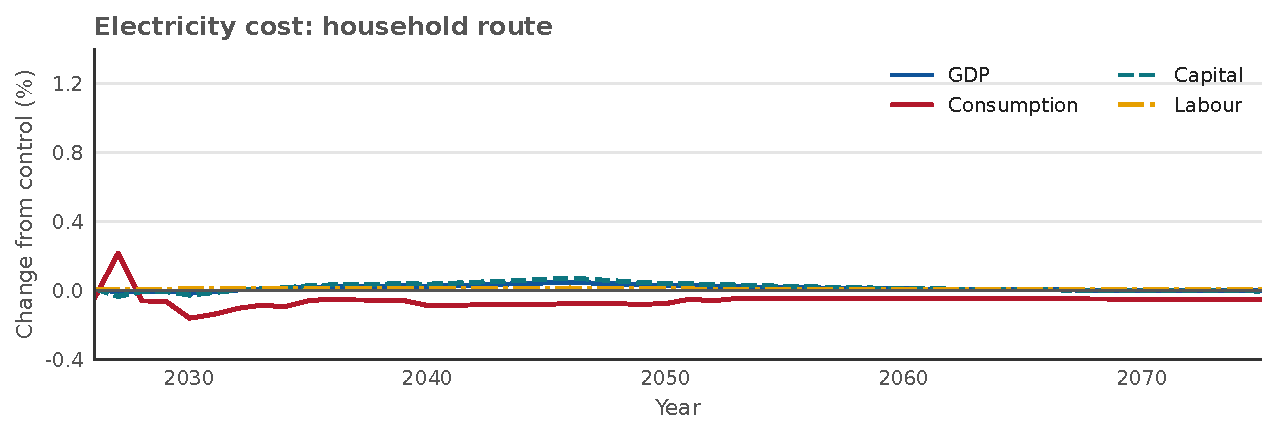
\includegraphics[width=\linewidth]{channel-macro-energy_price.pdf}
\caption{Electricity cost: the standalone household-price experiment. The affected
consumption good combines energy and water. This test does not include the industry
route or the revenue offset used in the combined case.}
\label{fig:electricity}
\end{figure}

\subsection{Public infrastructure investment}

Additional expenditure on assets designated as public enters government investment.
A publicly financed grid expansion adds productive infrastructure and creates a claim
on the public budget. The assessment weighs that benefit against taxes, debt or other
financing, including their effects on households and private investment.

The example mainly shifts expenditure between years, rather than adding a large
investment programme. Annual public investment varies between about 1.34\% below
and 0.37\% above the control; the public-capital stock peaks only 0.12\% above it.
The aggregate response is correspondingly small (Figure~\ref{fig:public-investment}).
Ownership and financing are specified, not inferred from the asset type.

\begin{figure}[H]
\centering
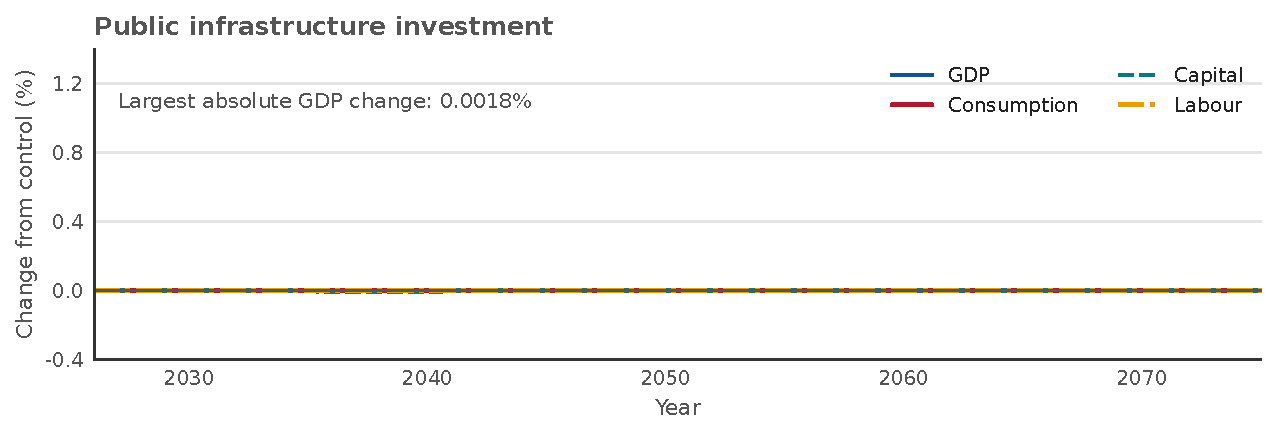
\includegraphics[width=\linewidth]{channel-macro-investment.pdf}
\caption{Public investment: the temporary change in spending produces little
aggregate movement on the common scale. The largest absolute GDP change is about
0.0018\%; this is a small scenario adjustment, not a general result about public investment.}
\label{fig:public-investment}
\end{figure}

\subsection{Generation capital intensity}

A different generation mix changes the role of capital relative to labour in electricity
production. The link uses the fleet's capital-cost share as a guide to that change in
OG-Core, rather than imposing an investment amount.

In the standalone example, the electricity industry's capital share rises from
78.2\% to 80.2\%. In the long run, electricity output rises by 4.4\%, while the
industry's capital use falls by 4.8\% and labour input by 18.7\%. Prices, output and
financing costs adjust together: changing production structure is not simply an
increase in investment. The aggregate chart (Figure~\ref{fig:capital-intensity})
shows little GDP movement despite that sectoral reallocation; consumption responds
more strongly during the transition.

\begin{figure}[H]
\centering
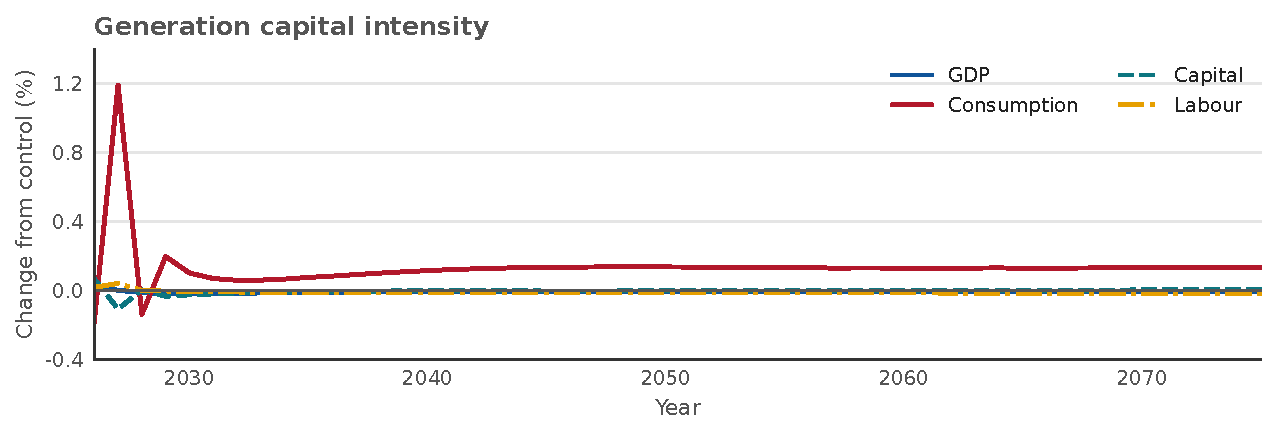
\includegraphics[width=\linewidth]{channel-macro-capital_intensity.pdf}
\caption{Capital intensity: aggregate responses to the changed electricity
production structure. The capital and labour lines cover the economy, not just
electricity; labour is an input measure, not a count of jobs.}
\label{fig:capital-intensity}
\end{figure}

\subsection{Air pollution and health}

Cleaner air can reduce premature deaths and illness. The link uses changes in
pollution, exposure assumptions and country health data to adjust survival rates
and working capacity by age. OG-Core then follows the resulting changes in population,
labour supply, consumption and saving.

In the standalone example, GDP and consumption are about 0.20\% and 0.24\% higher
on average over the first ten years. The response changes as the population adjusts:
labour eventually falls below the control even while output remains higher over the
period shown (Figure~\ref{fig:health-outcomes}). These are the survival and illness
effects together. Better health and longer life also have value beyond their
contribution to measured production and consumption.

\begin{figure}[H]
\centering
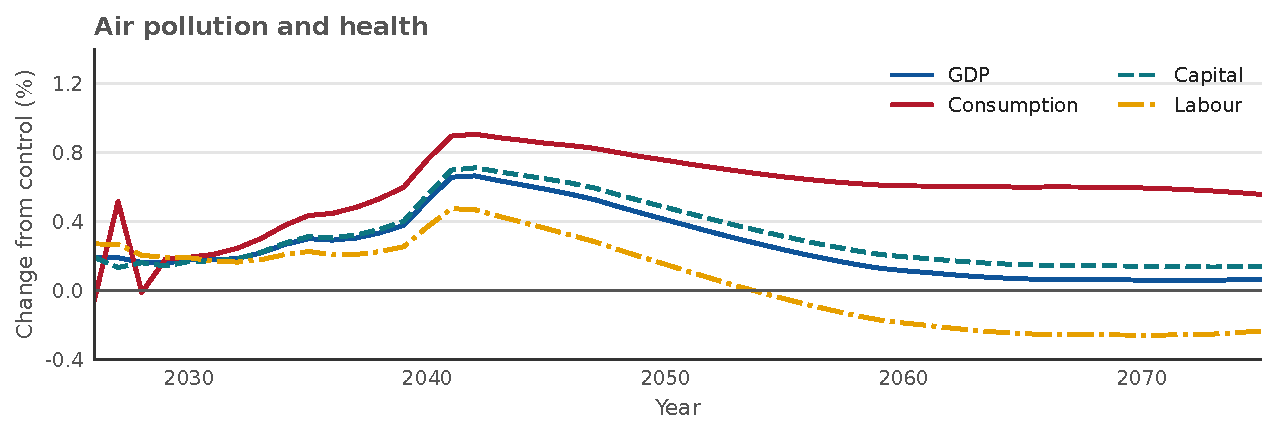
\includegraphics[width=\linewidth]{channel-macro-health.pdf}
\caption{Health: economic responses to the survival and working-capacity
adjustments in the standalone experiment. These are not estimates of the monetary
value of avoided illness or longer life.}
\label{fig:health-outcomes}
\end{figure}

\section{Policy Inputs and the Return to CLEWS}
\label{sec:illustration}

\subsection{Carbon price}

An exogenous carbon-price path can enter CLEWS as an emissions penalty. It can also enter
OG-Core as a payment on household energy use when that expenditure has not already been
priced through the electricity-cost ratio. Revenue can then be returned through household
transfers or used elsewhere in the public budget.

The same carbon cost cannot enter twice. If the carbon penalty has already changed the
CLEWS generation plan and is embodied in the electricity-cost ratio, OG-Core does not add
it again to the same electricity expenditure. Industrial carbon is represented through
CLEWS, because firms do not yet purchase an explicit energy input in OG-Core.

The carbon-price mapping has been tested on the economic side, and CLEWS can receive the
penalty path. The reported one-pass results do not include a CLEWS re-solve under that
policy path, so the carbon price has not yet changed the reported technology mix. Its
monetary magnitude also depends on the unfinished unit conversion.

\subsection{Private investment incentive}

The link can represent support for private generation investment through an investment
tax credit or related change in business taxation. This lowers the electricity industry's
cost of capital and shifts its demand for private capital. It is economically distinct
from the generation capital-intensity relationship, which changes production shares but
does not subsidise investment.

The mapping has been exercised as a standalone validation lever
(Section~\ref{sec:policy}). Its use in application will also require a calibrated
monetary bridge and a policy specification that distinguishes the incentive from the
underlying generation investment.

\subsection{Equilibrium return}

After OG-Core solves, the link writes its equilibrium portfolio return as a candidate
CLEWS discount rate. This can align resource planning with the economy's opportunity cost
of capital: a lower rate gives more weight to the future operating savings of
capital-intensive, long-lived assets.

The two rates are not automatically equivalent. A planning rate may reflect social
objectives, while an equilibrium return reflects market conditions. Risk, tax treatment,
maturity, and real-versus-nominal conventions also differ. The link therefore exposes a
choice that analysts must harmonise; it does not determine the correct social discount
rate. The return path is emitted --- a $\cplEmitDRPct\%$ rate in the current coupled
run --- but has not yet been passed through a repeated solution.

\subsection{Economic activity and electricity demand}

OG-Core also writes changes in industry output or household consumption to a revised
CLEWS demand path. The relevant measure depends on the service: industrial electricity
should follow the industries that use it, while household demand should follow household
consumption rather than aggregate GDP.

This return path supplies the demand response that is absent within the current CLEWS
optimisation. Higher electricity costs may reduce use and therefore change the capacity
required. Investment and health effects may raise activity and demand in other periods.

The mechanism for copying a revised demand path into CLEWS, solving the model, and reading
the result back has been tested with a controlled demand change. The activity path emitted
by OG-Core --- a mean demand change of $\cplDemandMeanPct\%$ in the current coupled run ---
has not yet travelled through the complete outer loop. Convergence and the
propagation of uncertainty across repeated solutions therefore remain untested.

\clearpage
\section{The Channels Together}
\label{sec:policy}

The combined example brings together household and industry electricity costs,
public investment and health. Capital-intensity changes, private incentives and
the household carbon tax are not included. Figure~\ref{fig:combined-path} uses the
same outcomes and scale as the individual-channel charts.

Matched runs show how this result builds up. Electricity costs and public investment
alone reduce average GDP by about 0.19\% over the first ten years. Adding health
changes that to a small gain of about 0.02\%. This is the effect of adding health
to that particular scenario, not its effect in isolation. The standalone experiments
do not add up to the combined result: they include different channels and a narrower
household-only electricity treatment.

\begin{figure}[H]
\centering
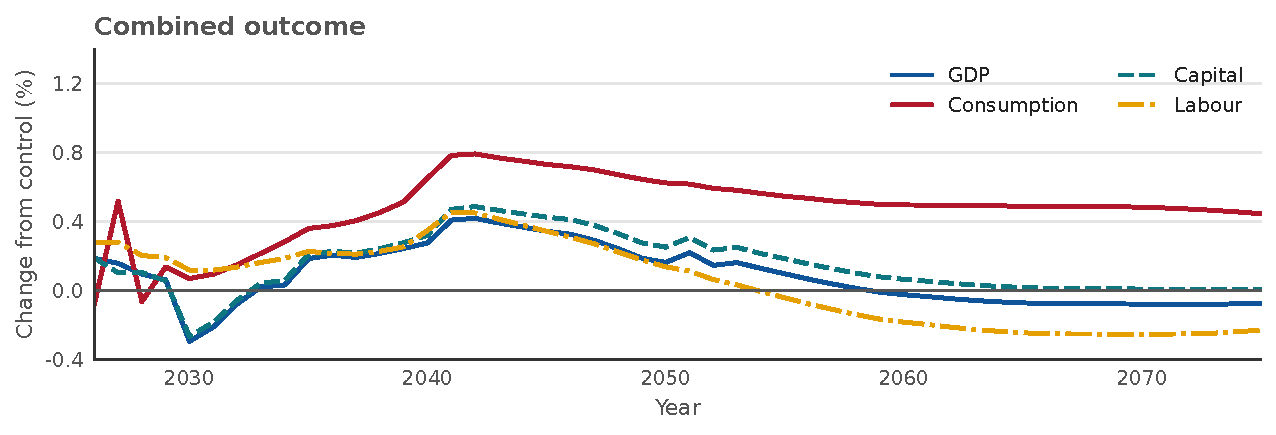
\includegraphics[width=\linewidth]{channel-macro-coupled.pdf}
\caption{Combined outcome: output, consumption, capital and labour over 2026--2075.
The comparison case, colours and scale are identical to the individual-channel
charts. The endpoint is 2075, not the eventual steady state.}
\label{fig:combined-path}
\end{figure}

The response changes over time. GDP falls below the control around 2030, recovers
to about 0.42\% above it in 2042, then falls below it again. Consumption remains
higher through the later years shown. Production, household consumption and the
timing of gains therefore need to be read together; the first-decade average does
not describe the whole adjustment.

These paths show the selected channels acting on the economy. The demand and
discount-rate signals have not yet been fed through a return CLEWS solve in this
example, so the charts do not show the subsequent revision of the resource plan.

\FloatBarrier
\section{Conclusion}
\label{sec:conclusion}

The OG--CLEWS link translates a solved resource strategy into the prices, investments,
health effects, and policy inputs that shape households, firms, government, and
different generations, and converts the resulting economic conditions back into inputs
for the next energy-model solve. Each relationship carries one mechanism, enters the
economy on one account, and can be inspected on its own, so a result can always be
traced back to the decision that produced it.

In the Philippine application, a decarbonisation
programme built around a coal moratorium from 2027 reshapes the power system while
leaving the economy moderately smaller in the long run: steady-state output changes by
$\cplYss\%$, with the adjustment carried mainly by wages ($\cplWss\%$) rather than
employment, and consumption by $\cplCss\%$. The same run converts a $\cplPMPct\%$
change in particulate exposure into roughly \cplDeaths{} avoided deaths and about
\cplMorbFTE{} full-time-equivalent workers per year of reduced illness. One
qualification travels with these numbers: nearly all of the output effect arrives
through the assumption that higher system costs pass into industry production costs,
and under the alternative productivity-based routing of the same cost signal the
aggregate sign reverses. The distributional account does not follow the familiar
budget-share intuition --- energy is a similar share of spending across income groups
here, so gains and losses are decided by earnings, assets, and transfers.

Three steps separate this system from application-grade policy numbers: a calibrated
monetary bridge, so that carbon and investment flows carry trusted units; a repeated
two-way solution, for which the mechanical seam is already tested; and a
country-calibrated health translation. Extending the same architecture to land and
water requires new resource-specific relationships and evidence, not a new method.


\bibliographystyle{plainnat}
\bibliography{../paper/references}

\end{document}
